\part{Vertices}
\frame{\partpage}

\begin{frame}{Interleaved Vertices}
	\begin{itemize}
		\pause\item Up until this point we have been storing vertex positions as floats
		\pause\item If we need a vertex to have colours, we can store these in a separate Vertex Buffer
		\pause\item Or we can create a \textbf{C structure} which represents a Vertex, which has member variables which represent positions, colours, normals etc
		\pause\item This is known as Interleaved Vertices and in \pause\textbf{MOST} cases is more efficient
	\end{itemize}
\end{frame}

\begin{frame}[fragile]{Vertex Structure 1}
	\begin{lstlisting}
		struct Vertex
		{
			float x,y,z;
		};
		
		Vertex v[]={{-0.5f,-0.5f,0.0f},
					{0.5f,-0.5f,0.0f},
					{0.0f,0.5f,0.0f}};
					 
	\end{lstlisting}
\end{frame}

\begin{frame}[fragile]{Vertex Structure 2}
	\begin{lstlisting}
		struct Vertex
		{
			float x,y,z;
			float r,g,b,a;
		};
		
		Vertex v[]={{-0.5f,-0.5f,0.0f,1.0f,0.0f,0.0f,1.0f},
					{0.5f,-0.5f,0.0f,0.0f,1.0f,0.0f,1.0f},
					{0.0f,0.5f,0.0f,0.0f,0.0f,1.0f,1.0f}};
	\end{lstlisting}
\end{frame}

\begin{frame}{Changes to the Vertex Buffer}
	\begin{itemize}
		\pause\item There will be a slight change to our vertex buffer
		\pause\item We have to take into account the size of the Vertex structure and the number of vertices in the buffer
	\end{itemize}
\end{frame}

\begin{frame}[fragile]{Vertex Buffer Changes - Old version}
	\begin{lstlisting}
		glBufferData(GL_ARRAY_BUFFER, sizeof(g_vertex_buffer_data), g_vertex_buffer_data, GL_STATIC_DRAW);
	\end{lstlisting}
\end{frame}

\begin{frame}[fragile]{Vertex Buffer Changes - new version}
	\begin{lstlisting}
		glBufferData(GL_ARRAY_BUFFER, 3* sizeof(Vertex), v, GL_STATIC_DRAW);
	\end{lstlisting}
\end{frame}

\begin{frame}{Changes to the Vertex Array}
	\begin{itemize}
		\pause\item Since the layout of the vertices have changed in memory, we need to update the Vertex Array Object to reflect this
		\pause\item Remember that the VAO describes the format of the vertices to the pipeline and enables the binding of vertex data to attributes in the shader 
	\end{itemize}
\end{frame}

\begin{frame}[fragile]{Vertex Array Object - Old version}
\begin{lstlisting}
	glEnableVertexAttribArray(0);
	glVertexAttribPointer(0,3,GL_FLOAT,GL_FALSE,0,(void*)0);
\end{lstlisting}
\end{frame}

\begin{frame}[fragile]{Vertex Array Object - New version}
\begin{lstlisting}
	glEnableVertexAttribArray(0);
	glVertexAttribPointer(0,3,GL_FLOAT,GL_FALSE,sizeof(Vertex),(void*)0);
	
	glEnableVertexAttribArray(1);
	glVertexAttribPointer(1,4,GL_FLOAT,GL_FALSE,sizeof(Vertex),(void*)(3*sizeof(float)));
\end{lstlisting}
\end{frame}

\begin{frame}{Memory and Vertex Array Object 1}
		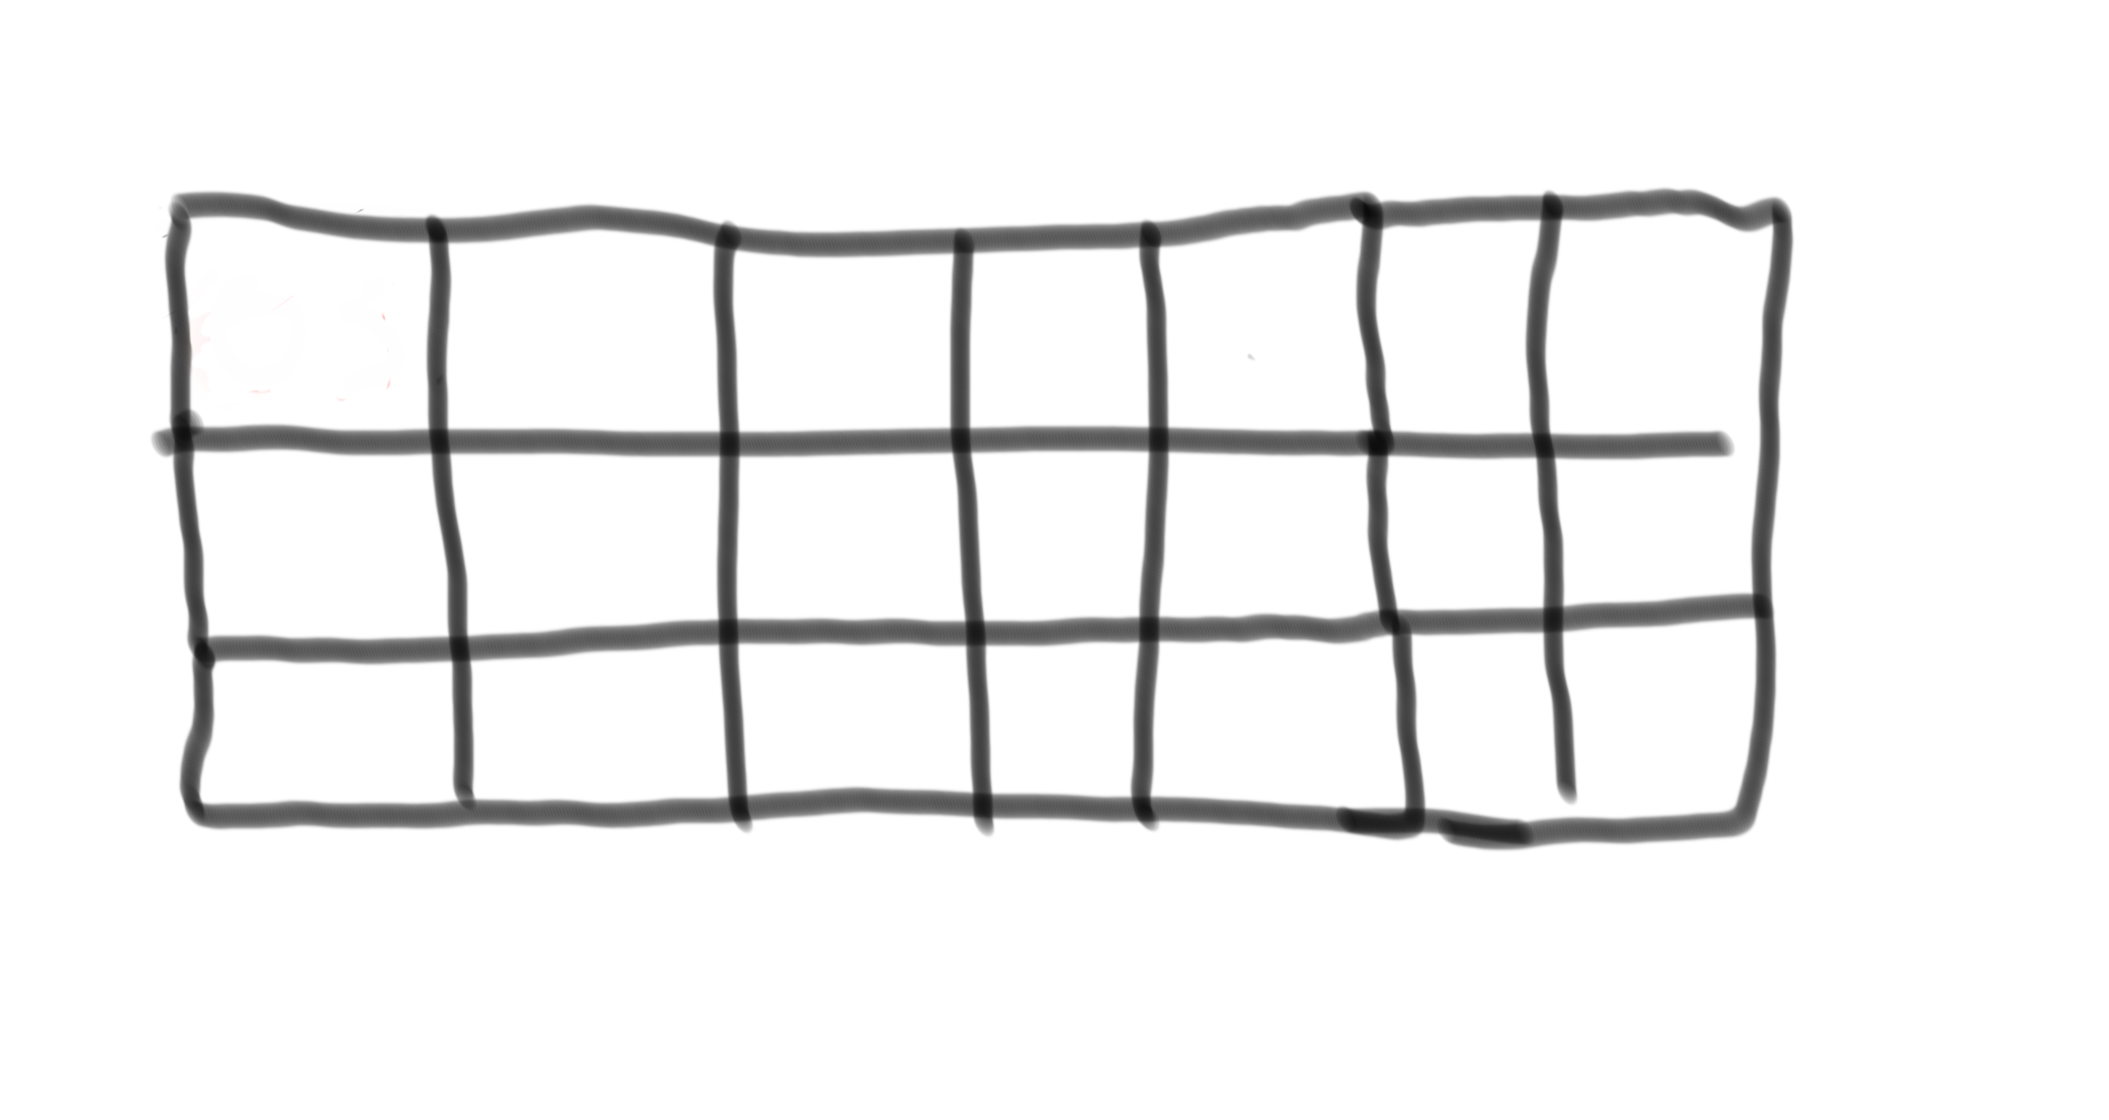
\includegraphics[width=1\textwidth]{MemoryLayoutStarter}	
\end{frame}

\begin{frame}{Memory and Vertex Array Object 2}
	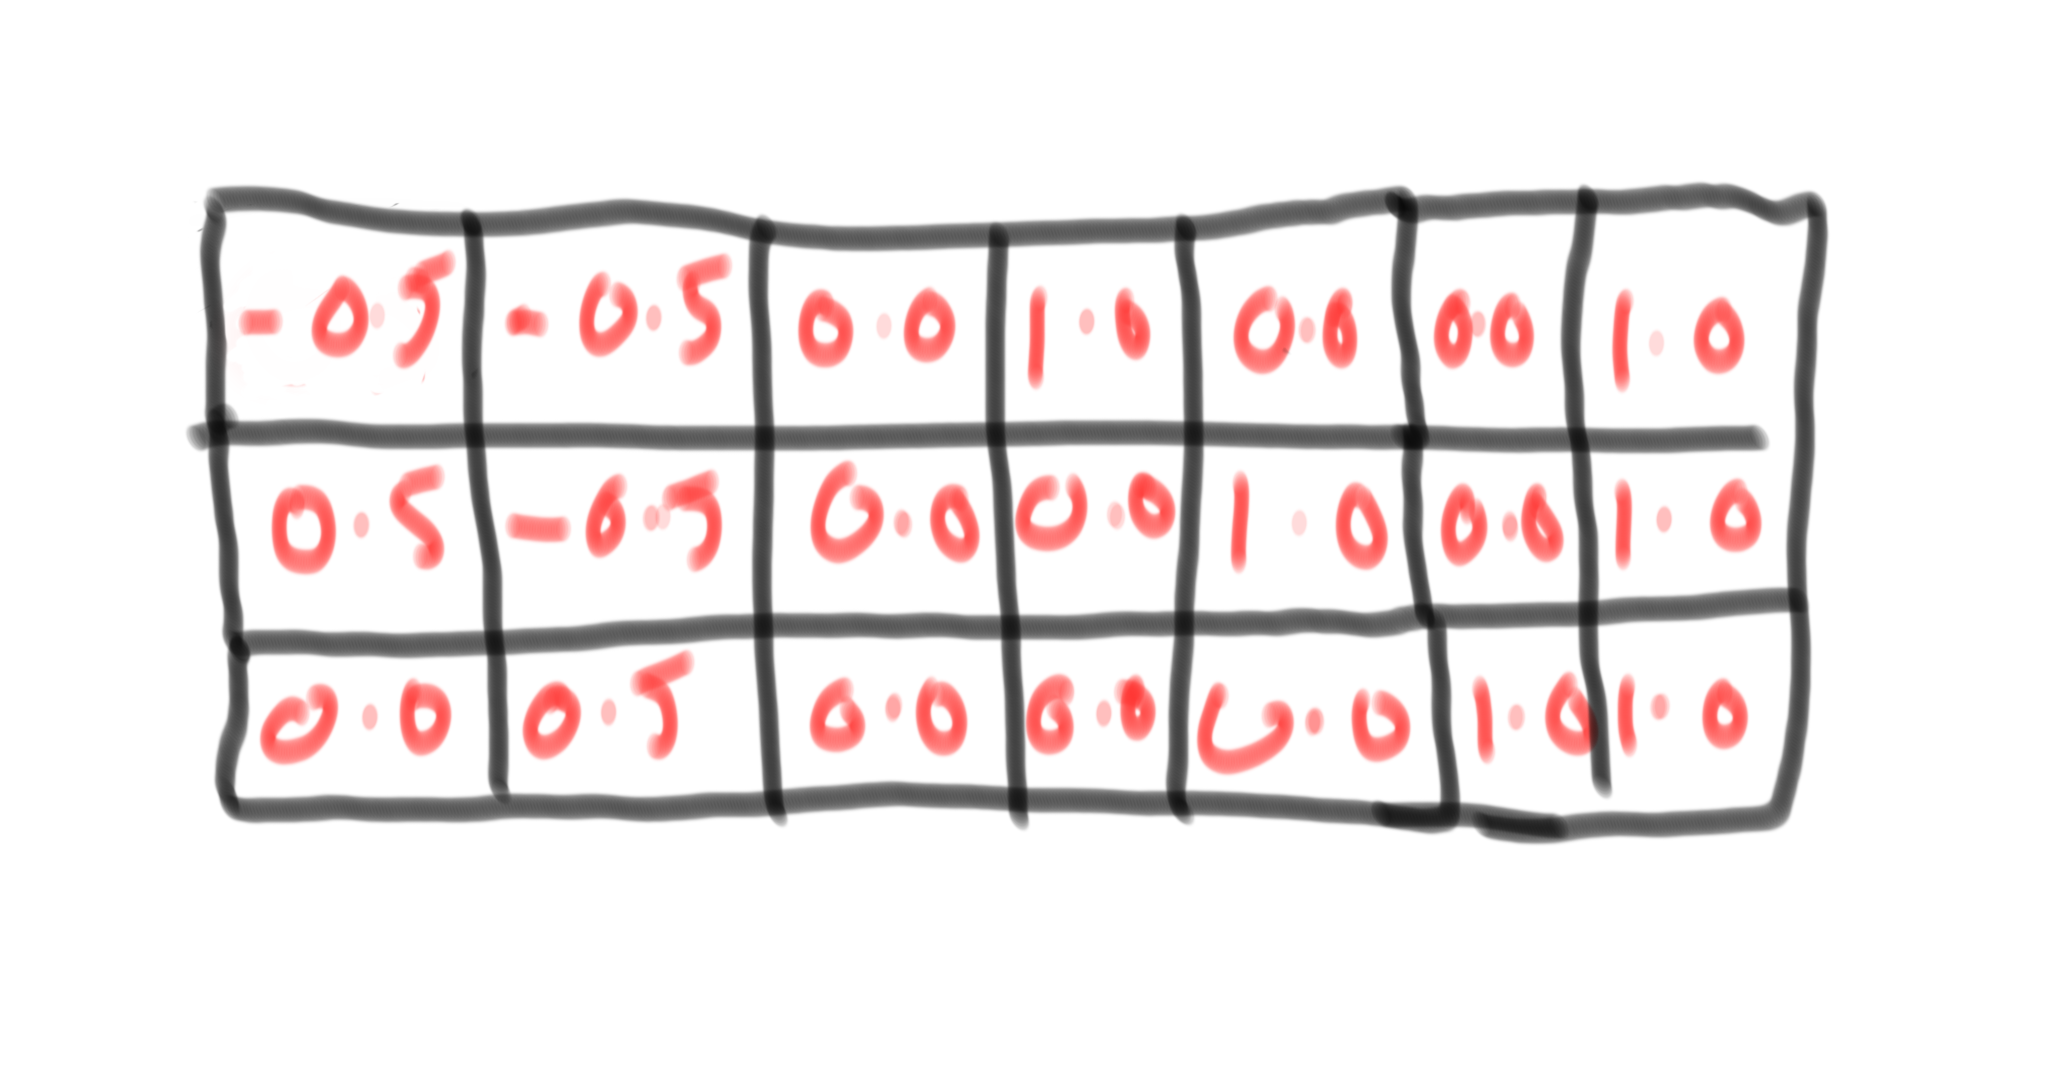
\includegraphics[width=1\textwidth]{MemoryLayoutValues}	
\end{frame}

\begin{frame}{Memory and Vertex Array Object 3 - Stride}
	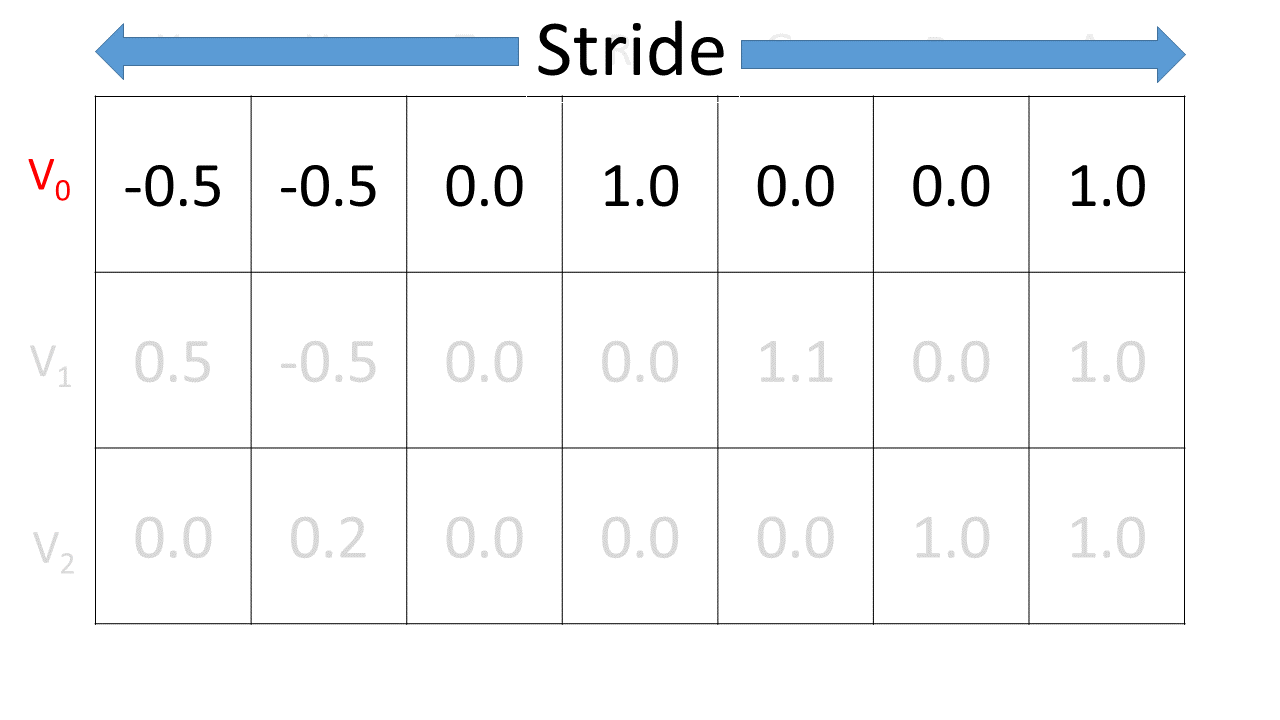
\includegraphics[width=1\textwidth]{MemoryLayoutStride}	
\end{frame}

\begin{frame}{Memory and Vertex Array Object 3 - Offset}
	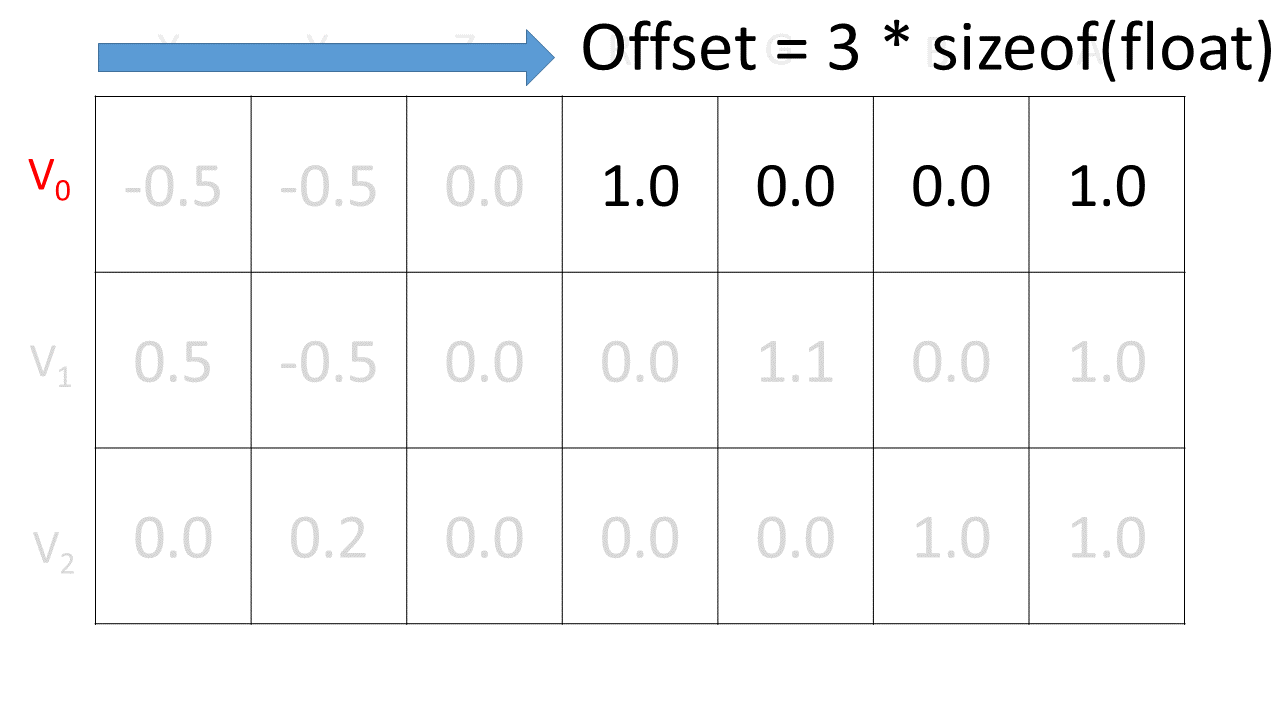
\includegraphics[width=1\textwidth]{MemoryLayoutOffset}	
\end{frame}